\documentclass[unicode,11pt,a4paper,oneside,numbers=endperiod,openany]{scrartcl}

\usepackage{ifthen}
\usepackage[utf8]{inputenc}
\usepackage{graphics}
\usepackage{graphicx}
\usepackage{hyperref}
\usepackage{amsmath}

\pagestyle{plain}
\voffset -5mm
\oddsidemargin  0mm
\evensidemargin -11mm
\marginparwidth 2cm
\marginparsep 0pt
\topmargin 0mm
\headheight 0pt
\headsep 0pt
\topskip 0pt        
\textheight 255mm
\textwidth 165mm

\newcommand{\duedate} {}
\newcommand{\setduedate}[1]{%
\renewcommand\duedate {Due date:~ #1}}
\newcommand\isassignment {false}
\newcommand{\setassignment}{\renewcommand\isassignment {true}}
\newcommand{\ifassignment}[1]{\ifthenelse{\boolean{\isassignment}}{#1}{}}
\newcommand{\ifnotassignment}[1]{\ifthenelse{\boolean{\isassignment}}{}{#1}}

\newcommand{\assignmentpolicy}{
\begin{table}[h]
\begin{center}
\scalebox{0.8} {%
\begin{tabular}{|p{0.02cm}p{16cm}|}
\hline
&\\
\multicolumn{2}{|c|}{\Large\textbf{Numerical Computing 2022 ---  Submission Instructions}}\\
\multicolumn{2}{|c|}{\large\textbf{(Please, notice that following instructions are mandatory: }}\\
\multicolumn{2}{|c|}{\large\textbf{submissions that don't comply with, won't be considered)}}\\
&\\
\textbullet & Assignments must be submitted to \href{https://www.icorsi.ch/course/view.php?id=14666}{iCorsi} (i.e. in electronic format).\\
\textbullet & Provide both executable package and sources (e.g. C/C++ files, Julia). 
If you are using libraries, please add them in the file. Sources must be organized in directories called:\\
\multicolumn{2}{|c|}{\textit{Project\_number\_lastname\_firstname}}\\
& and  the  file must be called:\\
\multicolumn{2}{|c|}{\textit{project\_number\_lastname\_firstname.zip}}\\
\multicolumn{2}{|c|}{\textit{project\_number\_lastname\_firstname.pdf}}\\
\textbullet &  The TAs will grade your project by reviewing your project write-up, and looking at the implementation you attempted, and benchmarking your code's performance.\\

\textbullet & You are allowed to discuss all questions with anyone you like; however: (i) your submission must list anyone you discussed problems with and (ii) you must write up your submission independently.\\
\hline
\end{tabular}
}
\end{center}
\end{table}
}
\newcommand{\punkte}[1]{\hspace{1ex}\emph{\mdseries\hfill(#1~\ifcase#1{Points}\or{Points}\else{Points}\fi)}}


\newcommand\serieheader[6]{
\thispagestyle{empty}%
\begin{flushleft}

\includegraphics[width=0.45\textwidth]{CI_logo}
\end{flushleft}
  \noindent%
  {\large\ignorespaces{\textbf{#1}}\hspace{\fill}\ignorespaces{ \textbf{#2}}}\\ \\%
  {\large\ignorespaces #3 \hspace{\fill}\ignorespaces #4}\\
  \noindent%
  \bigskip
  \hrule\par\bigskip\noindent%
  \bigskip {\ignorespaces {\Large{\textbf{#5}}}
  \hspace{\fill}\ignorespaces \large \ifthenelse{\boolean{\isassignment}}{\duedate}{#6}}
  \hrule\par\bigskip\noindent%  \linebreak
 }

\makeatletter
\def\enumerateMod{\ifnum \@enumdepth >3 \@toodeep\else
      \advance\@enumdepth \@ne
      \edef\@enumctr{enum\romannumeral\the\@enumdepth}\list
      {\csname label\@enumctr\endcsname}{\usecounter
        {\@enumctr}%%%? the following differs from "enumerate"
	\topsep0pt%
	\partopsep0pt%
	\itemsep0pt%
	\def\makelabel##1{\hss\llap{##1}}}\fi}
\let\endenumerateMod =\endlist
\makeatother




\usepackage{textcomp}


\usepackage{pgfplots} 
\usetikzlibrary{automata,topaths}

\makeatletter
\newcommand{\pgfplotsdrawaxis}{\pgfplots@draw@axis}
\makeatother
\pgfplotsset{only axis on top/.style={axis on top=false, after end axis/.code={
             \pgfplotsset{axis line style=opaque, ticklabel style=opaque, tick style=opaque,
                          grid=none}\pgfplotsdrawaxis}}}

\newcommand{\drawge}{-- (rel axis cs:1,0) -- (rel axis cs:1,1) -- (rel axis cs:0,1) \closedcycle}
\newcommand{\drawle}{-- (rel axis cs:1,1) -- (rel axis cs:1,0) -- (rel axis cs:0,0) \closedcycle}
\newenvironment{rcases}
  {\left.\begin{aligned}}
  {\end{aligned}\right\rbrace}


\begin{document}


\setassignment
\setduedate{Wednesday, December 21, 2022, 11:59 PM}

\serieheader{Numerical Computing}{2022}{Student: Albert Cerfeda}{}{Solution for Project 6}{}
\newline

\assignmentpolicy


The purpose of this project is to implement the Simplex Method to find the solution of linear programs, involving both the minimisation and the maximisation of the objective function.
\tableofcontents
\clearpage

\section{Graphical Solution of Linear Programming Problems [20 points]}
\subsection*{1.1 Minimization problem}
\begin{equation*}
    \begin{split}
    \text{min  } z & = 4x+y \\
     \text{\textbf{s.t}  } x+2y&\leq 40\\
     x+y&\geq 30 \\
     2x+3y&\geq 72 \\
     x,y &\geq 0
    \end{split}
\end{equation*}
Let us plot the inequalities on the Cartesian plane:\\
\begin{figure}[htpb] 
    \centering 
    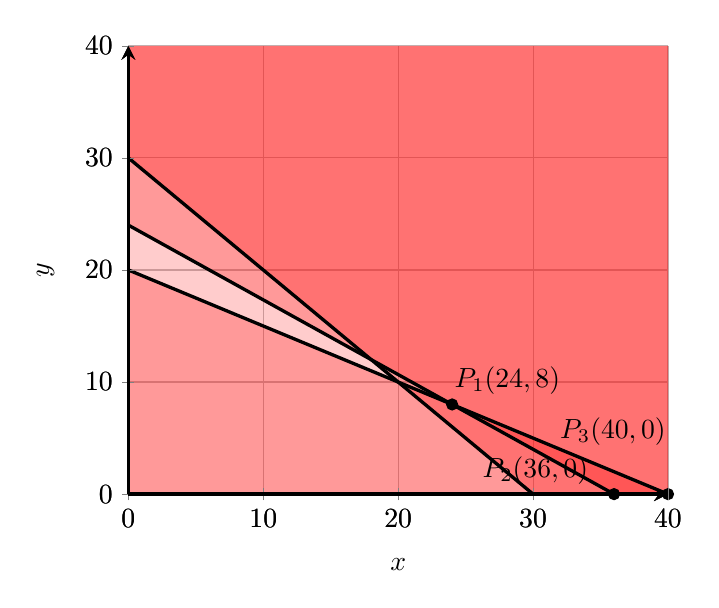
\begin{tikzpicture} 
      \begin{axis}[only axis on top,
        axis line style=very thick, 
        axis x line=bottom, 
        axis y line=left, 
         ymin=0,ymax=40,xmin=0,xmax=40, 
         xlabel=$x$, ylabel=$y$,grid=major 
      ] 
        
        \addplot [draw=none, fill=red, fill opacity=0.25, domain=-10:40]
        {(40-x)/2} \drawle; 
        \addplot [draw=none, fill=red, fill opacity=0.25, domain=-10:40]
        {30-x} \drawge;  
        \addplot [draw=none, fill=red, fill opacity=0.25, domain=-10:40]
        {(72-(2*x))/3} \drawge;
        \addplot [draw=none, fill=red, fill opacity=0.20, domain=-10:40]
        {0} \drawge;
        
        \addplot[very thick, domain=-10:40, ] {(40-x)/2} ; 
        \addplot[very thick, domain=-10:40, ] {30-x} ; 
        \addplot[very thick, domain=-10:40, ] {(72-(2*x))/3} ; 

        \addplot[mark=*,only marks] coordinates {(24,8)} node[above, xshift=0.7cm] {$P_1(24,8)$};
        \addplot[mark=*,only marks] coordinates {(36,0)} node[above, xshift=-1cm] {$P_2(36,0)$};
        \addplot[mark=*,only marks] coordinates {(40,0)} node[above, xshift=-0.7cm, yshift=0.5cm] {$P_3(40,0)$};
        

      \end{axis}
    \end{tikzpicture}
    \caption{Feasibile region for the Minimization problem} 
  \end{figure} 

We notice three intersection vertices:\\
\begin{tabular}{ ccc } 
    $x=24$ & $x=36,y=0$ & $x=40,y=0$\\
\end{tabular}\\
The point with $x=24$ is the intersection of inequalities $x+2y\leq 40$ and $2x+3y \geq 72$. Let's find the $y$ component of the intersection point:\\
$24+2y=40 \Rightarrow y=8$.\\\\
We now need to calculate the objective function value for each vertex:\\
\begin{tabular}{ ccc } 
    $p_1 = (24,8)$ & $p_2 = (36,0)$ & $p3=(40,0)$\\
\end{tabular}\\
\begin{equation*}
    \begin{split}
     z_1 &= 4(24)+ 8 = 104 \\
     z_2 &= 4(36) + 10 = 144 \\
     z_3 &= 4(40) + 0 = 160 \\
    \end{split}
\end{equation*}
Therefore $\text{min  } z = z_1 = 104$

\subsection*{1.2 Tailor maximisation problem}
The tailor in our problem sells two types of trousers, which we will identify as $x$ for the first type of trousers and $y$ for the second type of trousers.\\
The manufacturing cost of trouser $x$ equals $m_x = 25$ and for the case of trouser $y$ equals $m_y = 40$.\\
The retail price for trouser $x$ equals $85$  and for trouser $y$ equals $110$.\\
We denote the net profit for each trouser as $n_T$ where $T$ is the type of trouser. We can infer that $n_x=85-25=60$ and $n_y=110-40=70$.\\\\
\textbf{Note:} in the text of the exercise it is written \textit{The tailor estimates a total monthly demand of 265 trousers}. I interpreted it such that the tailor does not expect more than 365 trousers, i.e $x+y\leq265$. Were it to be intepreted as if the tailor was to expect at least 265 trousers, it would been have modeled with $x+y\geq265$.\\
Let us model the objective function aswell as the constraints:\\

% TODO: Plot constraints
\begin{equation*}
    \begin{split}
    \text{max  } z & = 60x+70y \\
     \text{\textbf{s.t}  } x+y&\leq 265\\
     25x+40y&\leq 7000 \\
     x,y &\geq 0, z\geq 0
    \end{split}
\end{equation*}\\
That is, the tailor wants to \textit{maximize} the net profit from selling both types of trousers, expects to sell not more than $265$ trousers, and spend less that $7000$ in raw materials.\\
The non-negativity constraints are intuitive as it is not possible to sell a negative amount of trousers.\\
Let's solve the systems of inequalities:\\
\begin{align*}
    & \begin{cases}
        y=0\\
        x+y=265
    \end{cases}\\
    &\begin{cases}
        y=0\\
        x=265
    \end{cases}\\
    &\Rightarrow P_1(265, 0) \\\\
    & \begin{cases}
        x+y=265\\
        25x+40y=7000
    \end{cases}\\
    &\begin{cases}
        x=265-y\\
        6625-25y+40y=7000
    \end{cases}\\
    &\begin{cases}
        x=265-y\\
        y=25
    \end{cases}\\
    &\Rightarrow P_2(240, 25)\\\\
    & \begin{cases}
        x=0\\
        40y=7000
    \end{cases}\\
    &\Rightarrow P_3(0, 175)
\end{align*}\\
Let's plot the inequalities on the Cartesian Plane:
\clearpage
\begin{figure}[h!] 
    \centering 
    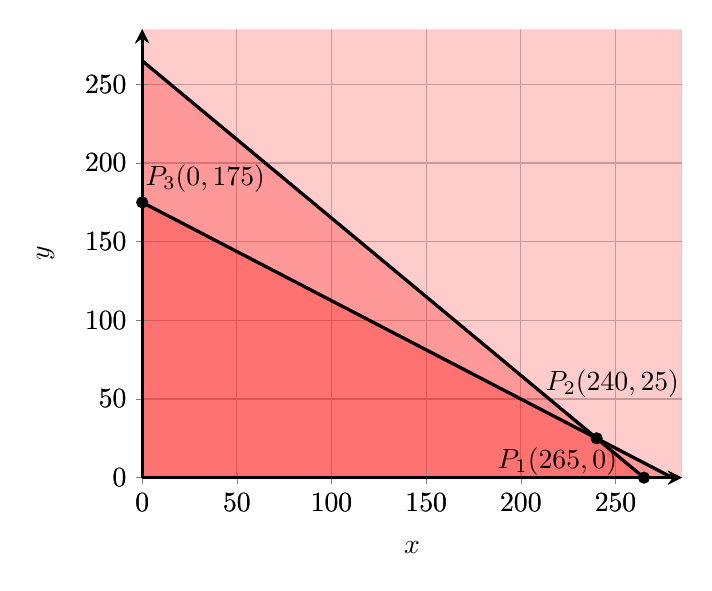
\begin{tikzpicture} 
      \begin{axis}[only axis on top,
        axis line style=very thick, 
        axis x line=bottom, 
        axis y line=left, 
         ymin=0,ymax=285,xmin=0,xmax=285, 
         xlabel=$x$, ylabel=$y$,grid=major 
      ] 
        
        \addplot [draw=none, fill=red, fill opacity=0.25, domain=-10:285]
        {265-x} \drawle; 
        \addplot [draw=none, fill=red, fill opacity=0.25, domain=-10:285]
        {(5*(-x+280))/8} \drawle;
        \addplot [draw=none, fill=red, fill opacity=0.20, domain=-10:285]
        {0} \drawge;
        
        \addplot[very thick, domain=-10:285, ] {265-x} ; 
        \addplot[very thick, domain=-10:285, ] {(5*(-x+280))/8} ; 

        \addplot[mark=*,only marks] coordinates {(265,0)} node[above, yshift=-0.1cm, xshift=-1.1cm] {$P_1(265,0)$};
        \addplot[mark=*,only marks] coordinates {(240,25)} node[above, yshift=0.4cm, xshift=0.2cm] {$P_2(240,25)$};
        \addplot[mark=*,only marks] coordinates {(0,175)} node[above, xshift=0.8cm, yshift=0cm] {$P_3(0,175)$};
        

      \end{axis} 
    \end{tikzpicture} 
    \caption{Feasible region for the Tailor maximisation problem} 
  \end{figure} 

\section{Implementation of the Simplex Method [30 points]}
The code has been successfully implemented in Julia.\\
When running the provided tests, all of them pass without incurring in the maximum iterations upper bound.\\
Please checkout the source files in the \verb|src/| folder, as it contains my implementation.

\section{Applications to Real-Life Example: Cargo Aircraft [25 points]}
\subsection*{3.1 Modelling the linear program}
Before modelling the linear problem we need to define the variable $t$:\\
$$
t_{xn} \text{where $x$ is the tonnes allocated from cargo $C_x$ and $n$ is the target Storage compartment $S_n$}
$$
There $t_14$ are the tonnes from Cargo 1 ie $C_1$ put into Storage compartment 4 ie $S_r$.
\begin{align*}
  \text{max} z &= (135*1*t_{11}) + (135*1.1*t_{12}) \\
  & +(200*1*t_{21})+(200*1.1*t_{22})\\
  & +(200*1.2*t_{23})+(200*1.3*t_{24})\\
  & +(410*1*t_{31})+(410*1.1*t_{32})\\
  & +(410*1.2*t_{33})+(410*1.3*t_{34})\\
  & +(520*1*t_{41})+(520*1.1*t_{42})\\
  & +(520*1.2*t_{43})+(520*1.3*t_{44})
\end{align*}
The objective function expresses the need to maximize the amount of profit from properly splitting the cargo in the available Storage compartments from the various Cargo containers.
\begin{align*}
  \text{\textbf{s.t. }} & \text{\textbf{Compartment weight capacity constraints}} \\
  & t_{11} + t_{21} + t_{31} + t_{45} \leq 18\\
  & t_{12} + t_{22} + t_{32} + t_{46} \leq 32\\
  & t_{13} + t_{23} + t_{33} + t_{47} \leq 25\\
  & t_{14} + t_{24} + t_{34} + t_{48} \leq 17\\
\end{align*}
Here we model the constraints coming from all the cargo loaded into the Storage compartment, not having to exceed the weight limit of the Storage compartment itself.
\begin{align*}
   & \text{\textbf{Compartment volume capacity constraints}} \\
  & 320*t_{11} + 510*t_{21} + 630*t_{31} + 125*t_{45} \leq 11930\\
  & 320*t_{12} + 510*t_{22} + 630*t_{32} + 125*t_{46} \leq 22552\\
  & 320*t_{13} + 510*t_{23} + 630*t_{33} + 125*t_{47} \leq 11209\\
  & 320*t_{14} + 510*t_{24} + 630*t_{34} + 125*t_{48} \leq 5870\\
\end{align*}
Here we model the constraints coming from all the cargo loaded into the Storage compartment, not having to exceed the volume limit of the Storage compartment itself.
\begin{align*}
  & \text{\textbf{Cargo volume availability constraints}} \\
  & (t_{11}+t_{12}+t_{13}+t_{14}) \leq 16\\
  & (t_{21}+t_{22}+t_{23}+t_{24}) \leq 32\\
  & (t_{31}+t_{32}+t_{33}+t_{34}) \leq 40\\
  & (t_{41}+t_{42}+t_{43}+t_{44}) \leq 28\\
\end{align*}
Here we model the maximum amount of cargo inside each container. Thus, we can't split more cargo than there actually is.
\begin{align*}
  & \text{\textbf{Non-negativity constraints}} \\
  & (t_{11}+t_{12}+t_{13}+t_{14}) \geq 0\\
  & (t_{21}+t_{22}+t_{23}+t_{24}) \geq 0\\
  & (t_{31}+t_{32}+t_{33}+t_{34}) \geq 0\\
  & (t_{41}+t_{42}+t_{43}+t_{44}) \geq 0\\
\end{align*}
Obviously the non-negativity constraints come from the impossibility of allocating a negative cargo weight.

\subsection{Solving the linear problem using Julia}
Let us model the problem in Julia for solving it:\\
% \begin{figure}[h!]
%   \begin{minted}[
%   frame=lines,
%   framesep=2mm,
%   linenos
%   ]{julia}
% cd(dirname(@__FILE__))
% include("simplex.jl")
% include("simplexSolve.jl")
% include("standardize.jl")
% include("auxiliary.jl")
% include("printSol.jl")

% function strcmp(str1, str2)
%     return cmp(str1, str2) == 0
% end

% # Input arguments:
% #   type = "max' for maximization; 'min" for minimization
% #   A    = matrix holding the constraints coefficients
% #   h    = coefficients of the constraints inequalities [rhs vector]
% #   c    = coefficients of the objective functions
% #   sign = vector holding information about the constraints if the system()
% #          needs to be standardized [-1: less or equal, 0: equal, 1:vgreater | equal]

% # Coefficient matrix A omitted
% # A ...

% type = "max"
% h = [ 18 32 25 17 11930 22552 11209 5870 16 32 40 28 ]'
% sign = [ -1 -1 -1 -1  -1 -1 -1 -1  -1 -1 -1 -1 ]
% c = [ 135 135*1.1 135*1.2 135*1.3    200 200*1.1 200*1.2 200*1.3    410 410*1.1 410*1.2 410*1.3    520 520*1.1 520*1.2 520*1.3]  
% z, x_B, index_B = simplex(type, A, h, c, sign)

% @show z, x_B, index_B
% \end{minted}
% \caption{Julia code for solving the real world linear problem for the Cargo Aircraft }
% \end{figure}

\textbf{Important}: Coefficient matrix A has been omitted from the report as it wouldnt have fit the page. Please check it out inside file \verb|src/exercise2.jl|.
The type has been set to "max" as this is a maximisation problem.
Matrix $A$ holds all the coefficients for the constraints, as modelled in the subsection before.
Vector $h$ contains all the right-hand sides of the constrain inequalities.
Vector $c$ contains all the coefficients of the objective function.
Vector $sign$ contains the information on whether each inequality sign has to be flipped. As this is a maximisation problem, and every explicit constraints inequality in our constraint is $\leq$, we have to flip all of them. 






\section{Cycling and Degeneracy [10 points]}



\end{document}
